\section{Experimental results}
% Bigger picture
There are many parameters involved in capturing the training images, extracting features, and training the random forest classifier. To study the contribution of these parameters, we systematically varied them and studied the accuracy of the resulting classifier. To study the accuracy, we set aside a collection of images as the test set and trained on a different set of images. We didn't use cross-validation due to the time constraints in training a random forest; it would have taken considerably longer time to test the cross validation accuracy and would  have prevented us from running as many tests as we did.

% Parameters tested
\subsection{Experiments}
We collected images of four different gestures shown in figure~\ref{fig:gestures}.

\textbf{Varying parameters.} We varied three parameters in training the models. We varied the number of trees in the forest from two trees to five trees; 1000, 2000 and 3000 features; and different number of training images starting at 10, 50, 100 up to 350 increments of 50. We also set aside 50 images as the test set. For each of these 96 configurations, we trained a random forest model and computed the test set accuracy.

The features represent randomly selected offsets from the point of prediction. The offsets are radially sampled up to a maximum radius. We varied the radius of the sampling and generated feature files. We trained models with 2000 features, three trees, and different number of training images for radii set to 20, 40, 60, 100 and 200. \todo{WHAT UNIT IS THIS???}.

Based on the results, we varied the parameters more in interesting directions: (1) We studied the effect of training a forest with just one tree and ten trees, (2) we trained with 689 training images, and (3) we tried smaller radii for the feature offsets. 

In addition to varying the parameters, we conducted three more experiments. 

\textbf{Randomness.} First, due to the nature of the random forest, the trained model is non-deterministic and may yield a different accuracy rate for the same training set of images. In order to study this randomness, we trained ten models on the the same training set with 1000 features, 300 training images, and one tree. 

\textbf{Pruning.} Second, we studied the effect of pruning on the accuracy of prediction. To study this, we pruned the forests trained with 2000 features and three trees for different number of training images. Then we calculated the test set accuracy of the pruned models.

\todo{SVM comparison.} Third, we evaluated random forest as a classification technique by comparing it to the error rates of a linear SVM. \todo{Explain more.}

We used the ALGLIB's random forest implementation for training and prediction \cite{alglib}. The experiments were run on high memory EC2 instances from Amazon, and a 48 GB server. \todo{Do we even have to mention this? Not very interesting.}


\subsection{Results}
\begin{figure}
\begin{center}
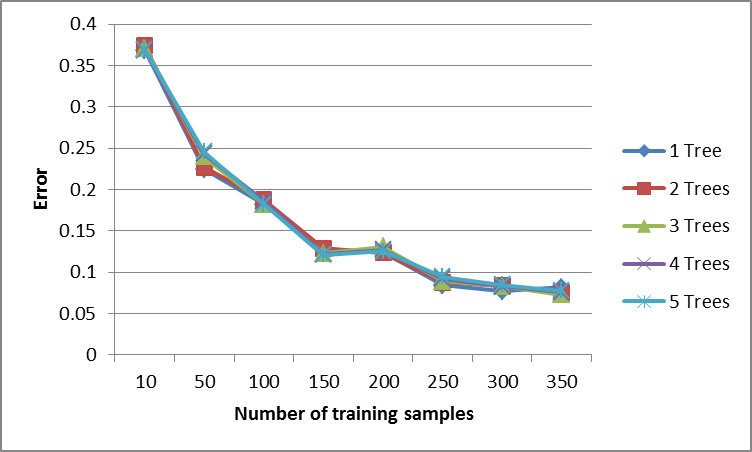
\includegraphics[width=0.45 \textwidth]{fig/varytrees.png}
\end{center}
\caption{Treeee}
\label{fig:varytrees}
\end{figure}

\begin{figure}
\begin{center}
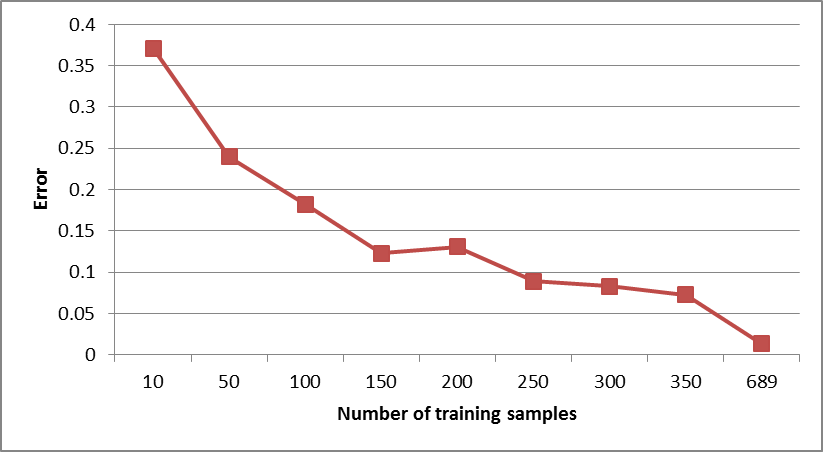
\includegraphics[width=0.45 \textwidth]{fig/largetraining.png}
\end{center}
\caption{TODO}
\label{fig:largetraining}
\end{figure}

\begin{figure}
\begin{center}
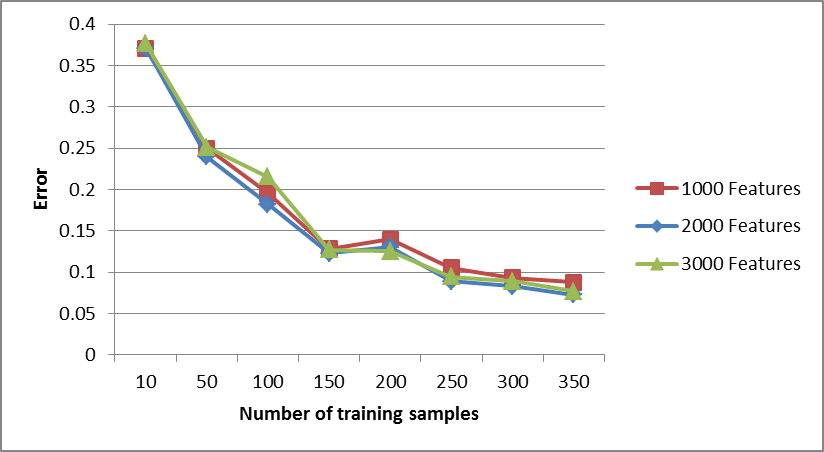
\includegraphics[width=0.45 \textwidth]{fig/varyfeatures.png}
\end{center}
\caption{TODO}
\label{fig:varyfeatures}
\end{figure}


\begin{figure}
\begin{center}
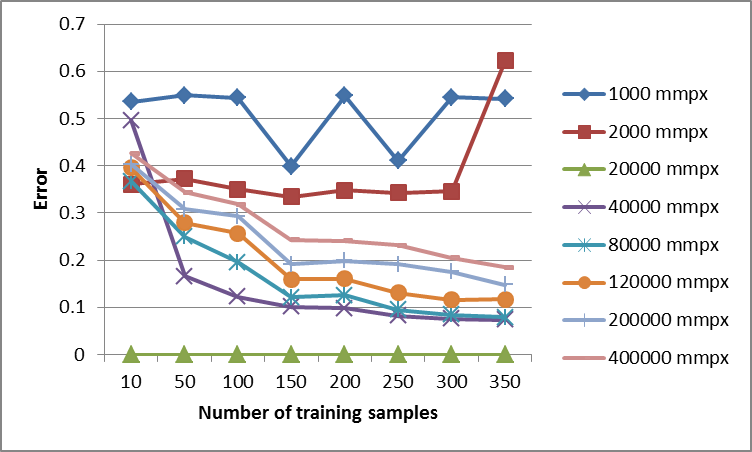
\includegraphics[width=0.45 \textwidth]{fig/varyradii.png}
\end{center}
\caption{TODO}
\label{fig:varyradii}
\end{figure}


\begin{figure}
\begin{center}
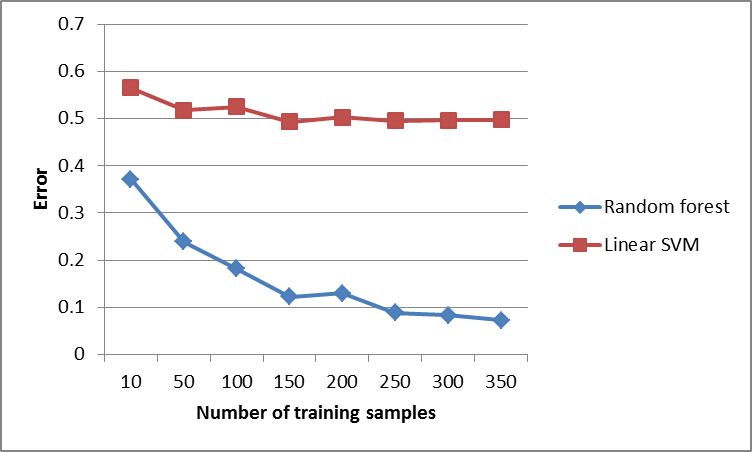
\includegraphics[width=0.45 \textwidth]{fig/linearsvm.png}
\end{center}
\caption{TODO}
\label{fig:linearsvm}
\end{figure}



\begin{figure}
\begin{center}
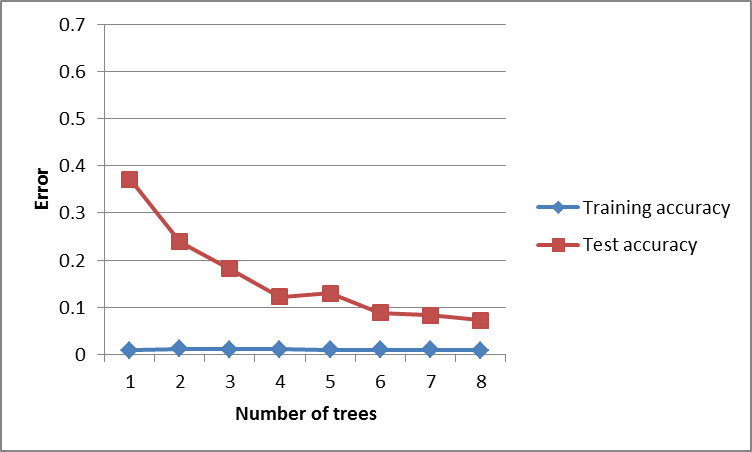
\includegraphics[width=0.45 \textwidth]{fig/trainingacc.png}
\end{center}
\caption{TODO}
\label{fig:trainingacc}
\end{figure}



\begin{itemize}
	\item \# of trees makes no difference! But kind of does in the practice. We think it has to do with the difference in background
	% 2000, 350, 1 - 10 trees x accuracy
	\item Increasing the training size makes the largest difference.
	% 2000, 3 trees, 10 - 689 x accuracy (or combine with above graph?)
	\item 2000 features does better than 3000 which does better than 1000.
	% 3 trees, 10 - 350 training x accuracy (3 curves for 1000, 2000, 3000)
	\item Decreasing the range leads to more accurate models faster. But as we increase the training size, it doesn't really matter.
	% 2000, 3 trees, 10 - 689 x accuracy (8 curves)
	\item The accuracy is roughly the same across multiple randomly trained models
	% Just report a number
	\item Pruning doesn't affect accuracy, which is great news for us.
	% Show this as overlapping plots, unless no space
	\item SVM
	\item Training accuracy for overfitting evidence
	\item The test accuracy doesn't seem to translate over the actual real-time prediction accuracy. This may be the different background.
\end{itemize}

So we built a wall.